\subsection{Define Precisely}

\subsubsection*{Iteration 1}

\paragraph*{Classification of Organizational Structures}

Figure \ref{fig:taxonomy} maps the organizational forms presented in Section \ref{sec:organizations} to the centralization axis, ranging them from highly centralized (e.g. bureaucratic) to decentralized (e.g. virtual organizations)

\begin{figure}
\centering
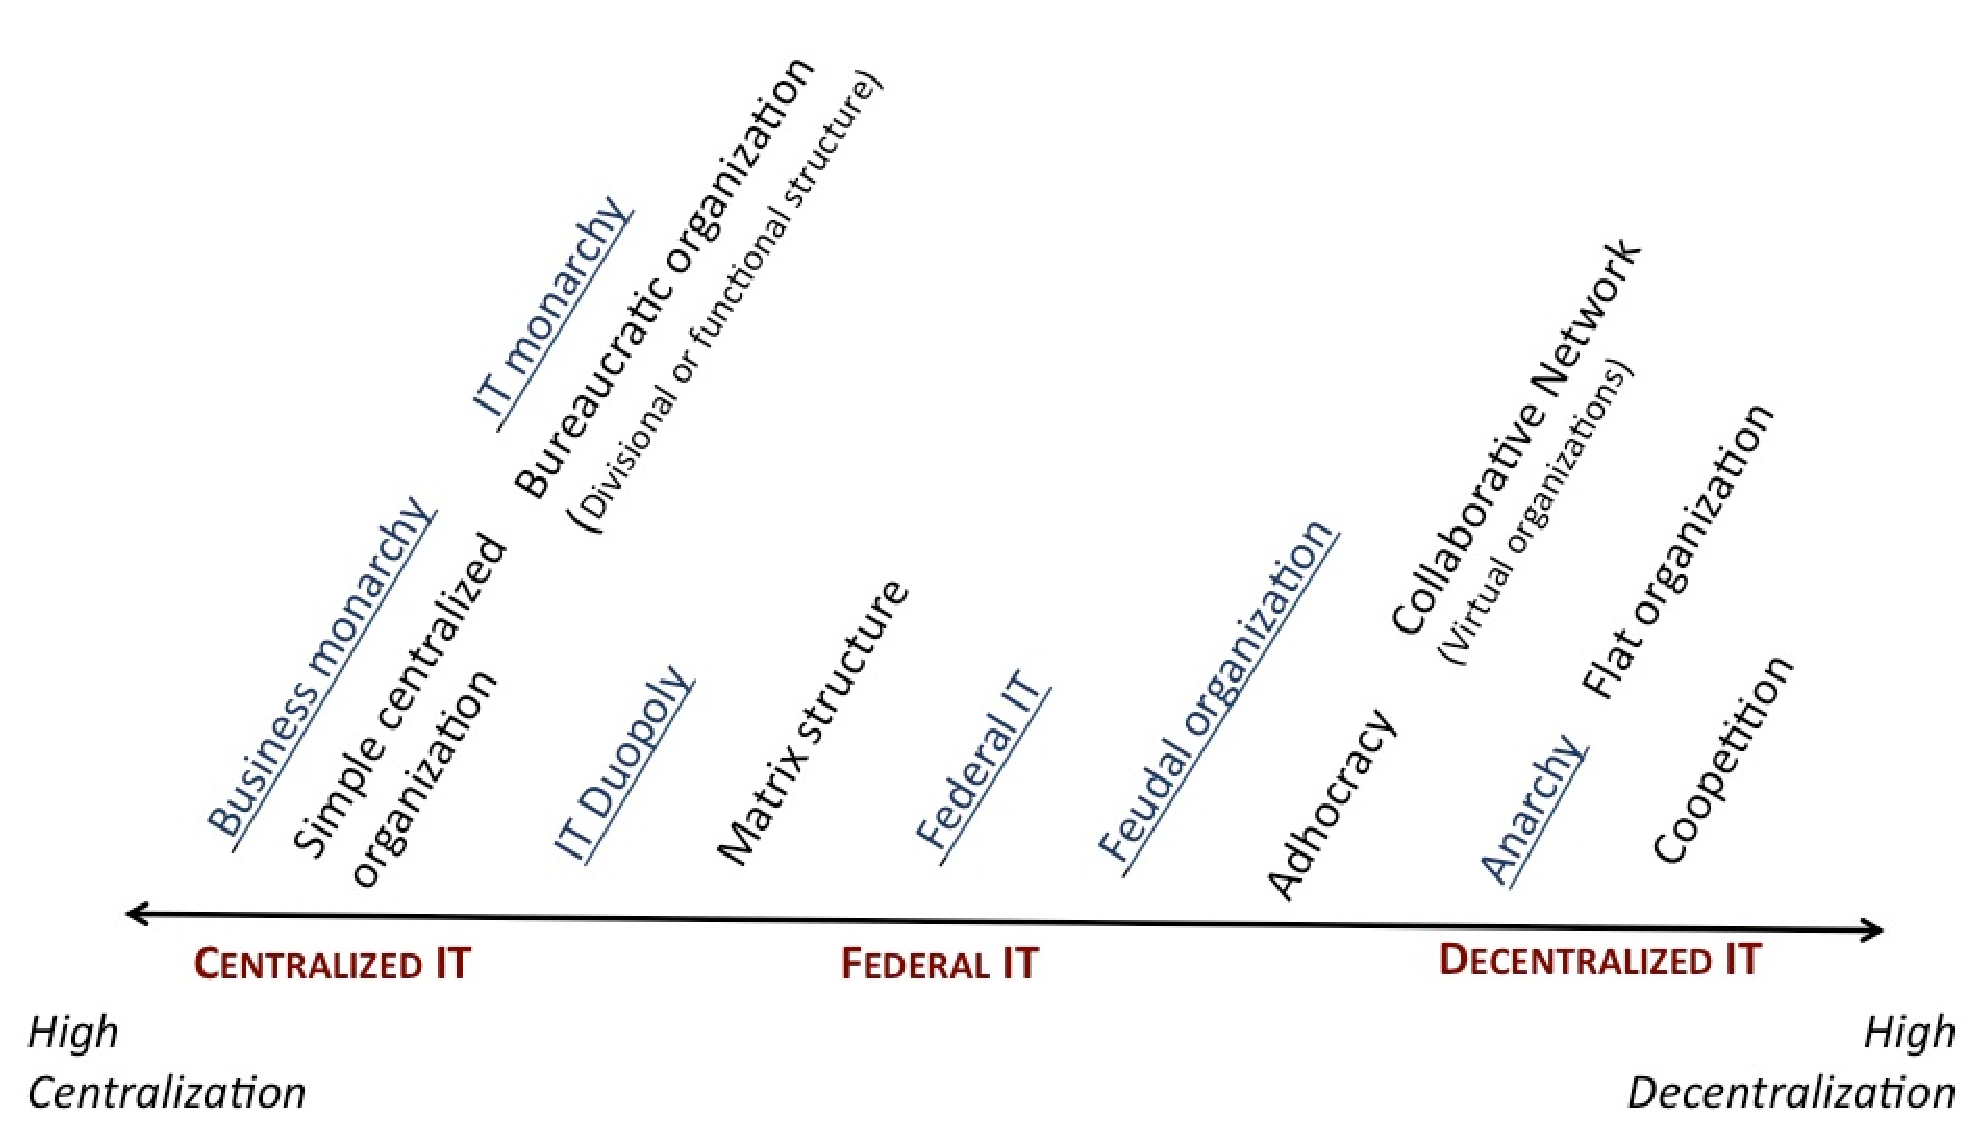
\includegraphics[scale=0.3]{taxonomy}
\caption{Organizational taxonomy: From Centralized to Decentralized}
\label{fig:taxonomy}
\end{figure}

\paragraph*{Role of EA}

Enterprise Architecture is a discipline  that allows an organization to construct and evolve its IT according to its needs. It provides a methodology and sets up a framework for assessing the current state of IT (architecture As-Is), for agreeing upon and communicating its future state (architecture To-Be), for planning, and for carrying out this transformation.

\paragraph*{The Problem (?)} 

It is important that  EA methodology and structures acknowledge progressive decentralization and help the organization to tackle the challenges related to it.    

more...
  

\subsubsection*{Iteration 2}

DSV has decent/federated structure, needs supporting EA

% **********************************************************************
% **********************************************************************
% **********************************************************************

\subsection{Motivate problem}

\subsubsection*{Iteration 1}

\paragraph*{Advantages of EA}

Why EA is good... 

\paragraph*{Key Differences Between Decentralized and Centralized Organizations}

Different organizational structures requires different EA...
 
Decentralized organizations face different challenges...
  
\subsubsection*{Iteration 2}

...

% **********************************************************************
% **********************************************************************
% **********************************************************************

\subsection{Find root causes}

\subsubsection*{Iteration 1}

\subsection{TOGAF}

\subsubsection{Concepts supporting a centralized organization}

\paragraph*{EA Method and EA Engine}
TOGAF outlines a formal approach to architecture governance which involves the setting up of an Architecture Board ``to oversee the implementation of the [architecture] strategy''~\cite[Ch. 47]{togaf9.1}. This board has an important role in Architecture Governance, such as ``[p]roviding the basis for all decision-making with regard to the architectures''~\cite[Ch. 47]{togaf9.1} and enforcing architecture compliance. 

%The TOGAF Architecture Governance Framework suggests guidelines for developing a formal governance structure for the Enterprise Continuum (and thus, all the architectural artifacts) and architecture processes. 

Architecture board concept suits well for the organization with strong centralization in IT (Centralized IT to Federal IT in Fig. \ref{fig:taxonomy}.  Having a single entity responsible for high-level decision making fits in with the concept of a Centralized IT organization. TOGAF does suggest that the board has enterprise-wide representation~\cite[Ch. 47]{togaf9.1} which may support some level of decentralization, however it suggests the representation comes in the form of ``senior managers''; a concept primarily from traditional organization structures. 

Throughout TOGAF, references are made to the existence of a bureaucratic or hierarchical centralized structure in place: 

For example, an important part of the preliminary phase [REF] is to set up a \textit{formal governance framework} for all architectural material, a concept that is related to the rigid forms of traditional organizational structure. 

Another example: after the completion of ``Phase A: Architecture Vision'', TOGAF requires approval of the current vision of the architecture. This requirement of approval assumes the existence of someone with a higher level of decision-making authority to give approval. 

A third example is an entire set of architectures at the strategic level of the Architecture Landscape which is meant for the ``executive level''~\cite[Ch. 20]{togaf9.1}.

\paragraph*{EA Description}
TOGAF suggests the development of architecture principles that ``...define the underlying general rules and guidelines for the use and deployment of all IT resources and assets across the enterprise''~\cite[Ch. 23]{togaf9.1}. Having a central set of principles that is to be applied to an entire organization supports centralization.

TOGAF includes the concept of an Architecture Repository, which is to hold the entirety of the Architecture Landscape in addition to other architecture-related information. The idea of a single place to store all information is highly supportive of centralization. 

\subsubsection{Concepts supporting decentralized organization}
\paragraph*{EA Method and EA Engine}
TOGAF primarily supports some level of decentralization through the concept of \textit{partitions}. It suggests dividing the Architecture Landscape into separate parts in order to support multiple architecture teams working concurrently and conflicting architectures in different organizational units. This enables ``federated architectures — independently developed, maintained, and managed architectures that are subsequently integrated within an integration framework''~\cite[Ch. 40.3]{togaf9.1}. 

Furthermore, ``[f]ederated architectures typically are used in governments and conglomerates, where the separate organizational units need separate architectures''~\cite[Ch. 40.3]{togaf9.1}. This supports the idea of different organizational units developing their own individual architectures. The mechanism for integrating the individual architectures under the roof of the corporate architecture is not explicit. 


TOGAF additionally indirectly supports decentralization through the suggestion that the entire TOGAF process be\textit{ tailored to fit the needs of the enterprise}. This is done in the preliminary phase of the ADM. In theory, this would allow TOGAF to support any kind of enterprise. The guidelines provided for this, however, are minimal. 

\subsection{Zachman}
%Limited perspectives?
\subsubsection{Concepts supporting centralized organization}

\paragraph*{EA Description}
The Zachman Framework aims to model a complete enterprise in a single, ``periodic table of elements''~\cite{Bente2012}. It attempts to break down an enterprise into a matrix of 36 elements, with alignment and composite integration relations defined between these elements. 

The perspectives of Zachman Framework line up with a bureaucratic organizational structure: the defined views (from executive to user) constitute an explicit organizational hierarchy. Clear separation between domains make this framework suitable for matrix organizations as well. 
%(e.g. executive and business management perspectives).

The lack of flexibility in definition of domains and views and the requirement to fill in the matrix - is perhaps the Zachman Frameworks main shortcoming with respect to decentralization. A primary aspect of decentralized organizations is their high level of flexibility. For a decentralized organization where both roles and domains are not uniformly defined (implicit) for sub-units, the use of the Zachman Framework becomes difficult if at all possible.

%Furthermore, the perspectives of Zachman Framework line up with a bureaucratic organizational structure (e.g. executive and business management perspectives). For a traditional, centralized organization these perspectives make a lot of sense. 

\paragraph*{EA Method and EA Engine}

Providing a schema for organizing architectural artifacts of an enterprise, the Zachman Framework does not imply any particular method for collecting these artifacts (what we call EA Method in Fig. \ref{fig:EA_general}).
Neither is suggests the set of structures that we call EA Engine. 

Therefore, tailoring and  implementation of Zachman framework for a concrete organizational structure depends on experience of the EA (consultancy) team.

To summarize, the Zachman Framework provides a detailed taxonomy of EA artifacts that supports a hierarchical view on the organization. The application of this framework in decentralized (flat, adhocracy) organizations remains unclear.

\subsection{FEA}
\subsubsection{Concepts supporting centralized organization}
\paragraph*{EA Description}
Through the use of a common set of \textit{reference models}, FEA prescribes standards that are to be followed throughout the organization. This limits the flexibility that the individual organizational units have and makes this framework suitable for bureaucratic organizations with a high level of standardization of its processes.

In FEA, however, individual organizational units have the freedom to develop their own architecture as long as it fits in to the set standards. This supports some level of decentralization and suits to organizations with federal structure, where individual units have input into decisions. 

\paragraph*{EA Method and EA Engine}

Segment architecture development is defined by FEA as a collaborative approach conducted by an integrated project team (IPT) comprising business subject matter experts, enterprise architects and technical subject matter experts.  FEA defines a set of segment architecture stakeholders and their roles (Table 2-2 in the document \cite{FEA_PMO2007}) in segment architecture development.   For example, the role of senior management is defined to set the agency strategic goals; chief architect and EA team are appointed to supervise the architecture development process, coordinate the activities of other stakeholders and communicate and share the information between segments when needed; IPT activities and meetings are coordinated and managed by a Program Manager. The Program Manager should monitor progress, evaluate segment architecture completion and demonstrate results. These roles naturally line up with the centralized to federal organization of IT (Fig.\ref{fig:taxonomy}).

According to FEA, ``Stakeholder commitment must be attained to support each step in this [development] process..''~\cite{FEA_PMO2007}.
 
The mechanism for integrating the segment architectures under the roof of the corporate architecture is  assured by specific governance and management processes, which are, tough implying different stakeholders, remain centralized. 

All steps of segment architecture development (Fig. \ref{fig:FEA_segmentDev}) involve/supervised by the Program manager and/or chief architect or Capital Planning and Investment Control (CPIC) lead, pointing on centralized management and budgeting.

Transition strategy is defined for the agency level though it is assessed on the global level. Governance-wide collaboration and reuse based on standards is outlined by FEA as an important part of RA transition strategy.

\subsubsection{Concepts supporting decentralized organization}
\paragraph*{EA Description}

The resulting segment architecture is positioned by FEA as a shared vision for business and IT transformation within a core mission area or common service. Each segment can have its own architecture that responds to its business needs.

\paragraph*{EA Method and EA Engine}

The development of \textit{segment architectures} is described as a collaborative process between EA architects and other stakeholders. The accent is placed on the ``reconciliation'' of the segment architecture with an agency architecture and cross-agency initiative, emphasizing the importance of  cross-agency collaboration, common opportunities and initiatives.

Architectural analysis and architectural definition steps of segment architecture development (Fig. \ref{fig:FEA_segmentDev}) involve business owners at the agency level who define business and information management requirements for the segment. This allows to ensure the local, agency-level interests within a corporation. 

FEA is targeting the groups of independent federal agencies with an objective to increase their inter-operability and quality of service they are offering for citizens. Among three EA methodologies considered in our study, FEA is the only one recognizing the need of inter- and intra-agency cooperation and communication. Nevertheless, many of the concepts on which the EA method and EA engine of FEA are grounded remain strongly centralized. Again, this supports our initial claim.

\begin{table*}
\caption{\textbf{ Existing and Prospective support of Progressive Decentralization by EA frameworks}}
\label{summary}
%%\begin{tabular}{l p{0.28\textwidth}}
\begin{tabular}{ | l | p{0.25\textwidth}| p{0.25\textwidth} | p{0.25\textwidth}|}
%
\hline
%
EA component: & 
\textbf{Existing support for centralized organizations} &
\textbf{Existing support for decentralized organizations} &  
\textbf{Applicable P2P principles for a solution} \\
%
\hline
%
\textbf{EA Method:} & 
Approval process based on hierarchy; architecture development is coordinated, supervised and evaluated by well-defined roles in a company (e.g. senior managers define strategic goals); EA teams coordinate architectural work and communicate results; results are controlled and evaluated centrally - by program manager) &
Federated architectures; possibility to adapt ADM for a specific organization; architecture development process involves multiple stakeholders & 
peer production principles for creation and evaluation of EA artifacts; P2P trust management replacing approval mechanism\\
%flexible ADM & peer production; P2P trust management\\
%
\hline
%
\textbf{EA Description:} & 
Strategic level architectures; hierarchy of architecture principles; a common set of reference models; hierarchical organization of EA artifacts with explicitly defined roles and domains (Zachman) &
Architecture partitions; architecture reference models; segment architecture; the concept of ``shared vision'' & 
User-driven content submission and change management of the content (i.e. the structure is defined by the users)\\
%
\hline
%
%
\textbf{EA Engine:} &
Architecture board; formal governance framework; common set of principles for entire organization (i.e global commitment is taken for granted); centrally managed architecture repository &
integration of various (segment) architectures is assured by (centralized) management and governance &
Peer production for relevance/accreditation (e.g. decision making in budgeting, strategy, opportunity evaluation, solution evaluation); user-driven content submission and change management of the content; P2P trust management\\
%
\hline
%
\end{tabular}
\end{table*}

\subsubsection*{Iteration 2}